\section{Introducción}

\subsection{Motivación}
\begin{frame}
  \frametitle{Motivación}
  \begin{enumerate}
    \item \textbf{La selección de características} es un procesamiento esencial en multitud de problemas relacionados con el aprendizaje automático.
    \item Existen muchos algoritmos y métodos para abordar este problema. En este proyecto, nos centraremos en las metaheurísticas.
    \item Se han propuesto muchos algoritmos metaheurísticos que se aplican a este problema. Tanto versiones con codificación real como binaria.
    \item Pese al gran número de algoritmos y versiones, no existen apenas comparaciones entre ellas.
  \end{enumerate}
  \vspace{-.2cm}
\end{frame}

\begin{frame}
  \frametitle{Motivación}
  \begin{enumerate}
    \item Este proyecto pretende hacer comparaciones rigurosas entre algoritmos.
    \item Comparaciones a nivel de distintas métricas, tales como el \textit{accuracy} o la reducción de características.
    \item Uso de test estadísticos robustos.
    \item Con el fin de dar la información más precisa sobre los algoritmos metaheurísticos en este problema.
  \end{enumerate}
  \vspace{-.2cm}
\end{frame}

\note{

}

\subsection{Contexto}
\begin{frame}
  \frametitle{Introducción a la Selección de Características}
  \begin{columns}
    \column{0.5\textwidth}
    \begin{enumerate}
      \item \textbf{La selección de características} es un proceso crucial en el aprendizaje automático.
            \begin{itemize}
              \item Implica elegir un subconjunto de características relevantes.
              \item Es un problema \textbf{NP duro}.
            \end{itemize}
            \item{Importancia de la reducción de dimensionalidad}:
            \begin{itemize}
              \item Mejora la generalización y precisión del modelo.
              \item Reduce el ruido en los datos.
            \end{itemize}
    \end{enumerate}
    \column{0.5\textwidth}
    \begin{figure}
      \begin{center}
        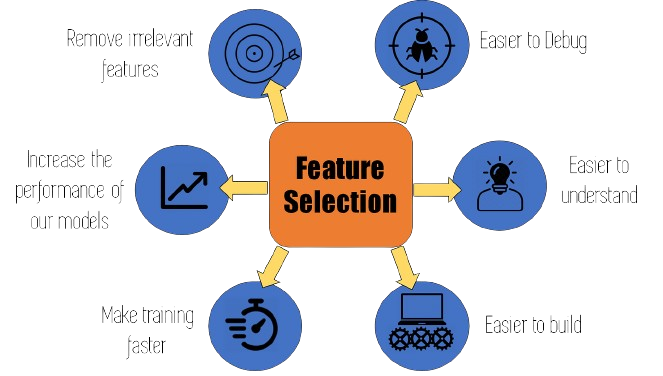
\includegraphics[width=\textwidth]{imagenes/chapter1/feature_selection_pros-removebg-preview.png}
      \end{center}
      \caption{Beneficios de la selección de características}
    \end{figure}
  \end{columns}
  \vspace{-.2cm}
\end{frame}

\note{

}

\subsection{Objetivos}
\begin{frame}
  \frametitle{Objetivos}
  \begin{columns}
    \column{0.6\textwidth}
    \begin{enumerate}
      \item Evaluar el desempeño de las metaheurísticas.
      \item Investigar versiones continuas y binarias.
      \item Fortalezas y debilidades de las metaheurísticas.
      \item Recomendaciones prácticas según el contexto.
      \item Evaluación de resultados finales y realizar comparaciones.
      \item Resolver una serie de preguntas de investigación. ¿Binarios vs continuos?
    \end{enumerate}
    \column{0.6\textwidth}
    \begin{figure}
      \begin{center}
        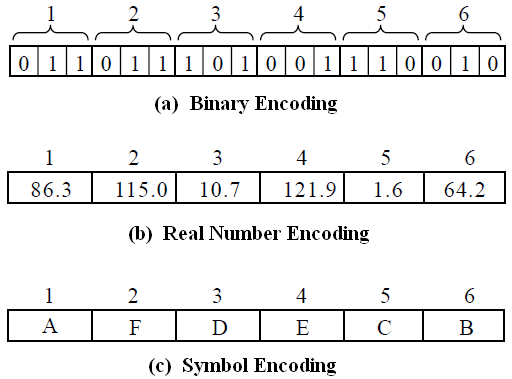
\includegraphics[width=0.7\textwidth]{imagenes/chapter1/real_vs_bin.png}
      \end{center}
      \caption{Codificaciones binarias y continuas\footnotemark[1]}
    \end{figure}
  \end{columns}
  \footnotetext[1]{\cite{binary_real}}
\end{frame}

\note{

}

\subsection{Metaheurísticas}
\begin{frame}
  \frametitle{¿Qué son las metaheurísticas?}
  \begin{columns}
    \column{0.6\textwidth}
    \begin{enumerate}
      \item Las metaheurísticas son algoritmos de \textbf{optimización}.
      \item Suelen estar bioinspiradas.
      \item Son algoritmos generales que no dependen de un dominio en un problema específico.
      \item Consiguen soluciones muy buenas en tiempos razonables.
    \end{enumerate}
    \column{0.4\textwidth}
    \begin{figure}
      \begin{center}
        \animategraphics[loop, autoplay, width=0.8\textwidth]{10}{imagenes/chapter1/ParticleSwarmArrowsAnimation-}{0}{99}
      \end{center}
      \caption{Algoritmo PSO en busca del \textbf{mínimo} de una función\footnotemark[2]}
    \end{figure}
  \end{columns}
  \footnotetext[2]{\cite{wiki:PSO}}
\end{frame}

\note{

}

\begin{frame}
  \frametitle{Tipos de mateheurísticas}
  \begin{columns}
    \column{0.4\textwidth}
    \begin{figure}
      \begin{center}
        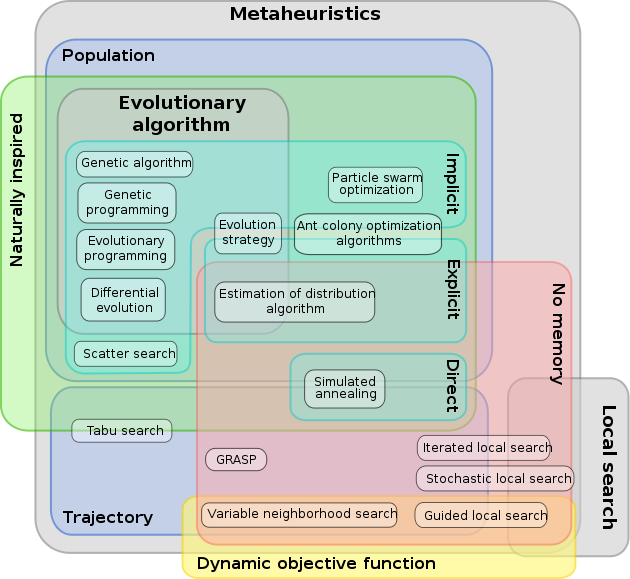
\includegraphics[width=1\textwidth]{imagenes/chapter1/mh_euler_graph.png}
      \end{center}
      \caption{Tipos de metaheurísticas}
    \end{figure}
    \column{0.6\textwidth}
    \begin{enumerate}
      \item Las metaheurísticas seleccionadas en este proyecto son todas del tipo \textbf{poblacional} y evolutivas.
    \end{enumerate}
  \end{columns}
\end{frame}

\note{

}


\note{

}